\begin{figure}[htbp]
	% Partly taken from http://www.texample.net/tikz/examples/convolution-of-two-functions/
	\centering
	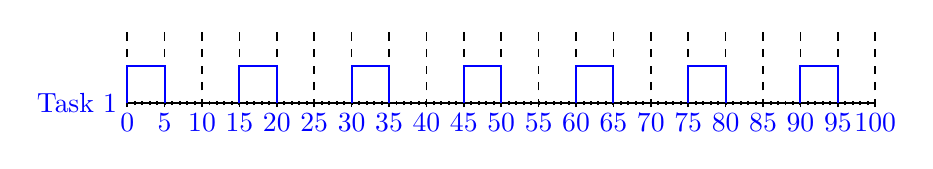
\begin{tikzpicture}[
		scale=0.095,
		line width=0.25mm,
		every node/.style={scale=1, text=blue},
		major tick/.style={semithick, dashed},
		x tick label/.style={anchor=north, minimum width=5mm},
		task1/.style={blue},
		task2/.style={red},
		task3/.style={green},
		desc/.style={anchor=east}
		]
	
	% Task 1
	\draw (0, 0) -- (100, 0);
	\node[desc] at (0, 0) {Task 1};
	
%	% Task 2
%	\draw (0, 10) -- (100, 10);
%	\node[desc] at (0, 10) {Task 2};	
%	
%	% Task 3
%	\draw (0, 20) -- (100, 20);
%	\node[desc] at (0, 20) {Task 3};	
	
	% Small ticks
	\foreach \x in {0, 1,...,100}{
		\draw (\x, -0.25) -- (\x, 0.25);
	}
	
	% Major ticks with label
	\foreach \x/\label in {0, 5,...,100}{
		\node[x tick label] at (\x, 0) {$\label$}; 		
		\draw[major tick] (\x, -0.5) -- (\x, 10);
	}
	
	% Draw all
%	\foreach \x in {0, 15,...,100}{
%		\draw[task1] (\x, 0) -- (\x, 5) -- (\x+5, 5) -- (\x+5, 0);
%	}
	
	% Single steps for the slides
	\draw[task1] (0, 0) -- (0, 5) -- (5, 5) -- (5, 0);
	\draw[task1] (15, 0) -- (15, 5) -- (20, 5) -- (20, 0);
	\draw[task1] (30, 0) -- (30, 5) -- (35, 5) -- (35, 0);
	\draw[task1] (45, 0) -- (45, 5) -- (50, 5) -- (50, 0);
	\draw[task1] (60, 0) -- (60, 5) -- (65, 5) -- (65, 0);
	\draw[task1] (75, 0) -- (75, 5) -- (80, 5) -- (80, 0);
	\draw[task1] (90, 0) -- (90, 5) -- (95, 5) -- (95, 0);

	\end{tikzpicture}
\end{figure}